\documentclass[10pt]{article}

% Final version: use atml without [instructions]
\usepackage{atml}

\input{math_commands.tex}

\usepackage{hyperref}
\usepackage{url}
\usepackage{graphicx}
\usepackage{booktabs}
\usepackage{float}
\usepackage{xcolor}

\title{Reproducibility Challenge: Generative Proxemics}

\author{%
  \name Nawfal Abdul Malick \email nawfal.malick@usi.ch
  \AND
  \name Teammate 1 Name \email teammate1@usi.ch
  \AND
  \name Teammate 2 Name \email teammate2@usi.ch
}

\def\groupid{GenProxemics}
\def\projectid{GenProxemics}

\begin{document}

\maketitle

\begin{abstract}
This report presents our reproducibility study of \emph{Generative Proxemics: A Prior for 3D Social Interaction from Images}. The paper introduces BUDDI, a diffusion-based prior for modelling and reconstructing two people in close physical interaction from images. Our group studied the main generation and reconstruction components of the method and added an extension that evaluates robustness under degraded BEV initialization. Due to access restrictions on the authors' processed FlickrCI3D auxiliary files, our Task 3 experiment could not use the official pseudo-ground-truth fits. Therefore, we adapted the extension into a qualitative robustness study. We successfully ran the BUDDI optimization pipeline on FlickrCI3D test images, generated clean BEV outputs, injected controlled noise into the BEV initialization, and reran BUDDI optimization across four noise levels.
\end{abstract}

\section{Introduction}

The original paper addresses the problem of reconstructing two interacting people in 3D from a single image. This setting is challenging because close human interaction often involves occlusion, physical contact, and ambiguous depth relationships. A method may reconstruct each person individually, but still fail to correctly model the spatial relation between them.

BUDDI is proposed as a learned prior for two-person proxemics. In this context, proxemics refers to the spatial arrangement and physical relationship between people during interaction. Instead of treating two bodies independently, BUDDI learns plausible configurations of two people in close proximity and uses this knowledge during reconstruction.

Our group divided the project into three parts. Task 1 studies generation and unconditional sampling. Task 2 focuses on optimization-based reconstruction and comparison with the original paper's reconstruction results. Task 3, which is my contribution, studies how BUDDI behaves when the initial BEV reconstruction is intentionally degraded.

\section{Scope of reproducibility}
\label{sec:claims}

We focus on the following claims and extension:

\begin{itemize}
    \item \textbf{Claim 1:} BUDDI can model realistic two-person 3D interactions.
    \item \textbf{Claim 2:} BUDDI can improve optimization-based reconstruction of interacting people from images when used as a prior.
    \item \textbf{Extension / Task 3:} If the BEV initialization is degraded, BUDDI should still be able to produce plausible two-person reconstructions because it provides a learned interaction prior.
\end{itemize}

Task 3 does not reproduce a specific table from the original paper. Instead, it tests an additional robustness question: how sensitive is BUDDI optimization to the quality of the initial BEV estimate?

\section{Methodology}

\subsection{Model descriptions}

The reconstruction pipeline consists of three main components.

\paragraph{ViTPose.}
ViTPose is used to detect 2D body keypoints in the input image. These keypoints provide image evidence during optimization.

\paragraph{BEV.}
BEV provides an initial 3D reconstruction of the detected people. In our Task 3 experiment, this component is especially important because we intentionally perturb its output to create degraded initializations.

\paragraph{BUDDI optimization.}
BUDDI is used as a learned prior during optimization. The purpose of this prior is to encourage plausible two-person configurations, especially in close interactions where independent body reconstruction methods may fail.

The overall pipeline is:
\[
\text{Image} \rightarrow \text{ViTPose keypoints} \rightarrow \text{BEV initialization} \rightarrow \text{BUDDI optimization}.
\]

\subsection{Datasets}

For Task 3, we used the original FlickrCI3D test images. The available data contained:

\begin{itemize}
    \item \texttt{FlickrCI3D\_Signatures/test/images}
    \item \texttt{interaction\_contact\_signature.json}
\end{itemize}

However, we could not access the authors' processed FlickrCI3D auxiliary files:

\begin{itemize}
    \item \texttt{processed.pkl}
    \item \texttt{processed\_pseudogt\_fits.pkl}
\end{itemize}

These files are important because they contain preprocessed inputs and pseudo-ground-truth SMPL-X fits. Without them, we could not compute the official PA-MPJPE or PCC metrics. Therefore, Task 3 was adapted into a qualitative robustness experiment rather than a full official quantitative evaluation.

\textcolor{blue}{\textbf{Task 1 placeholder:}} Teammate 1 should add the datasets used for generation and unconditional sampling here.

\textcolor{blue}{\textbf{Task 2 placeholder:}} Teammate 2 should add the datasets and evaluation splits used for reconstruction reproduction here.

\subsection{Task 3: BEV degradation robustness experiment}

The goal of Task 3 was to test whether BUDDI remains stable when the BEV initialization is degraded. We first ran the normal BUDDI pipeline on FlickrCI3D test images and obtained valid reconstructions for four detected two-person examples:

\begin{itemize}
    \item \texttt{flickr\_0057\_0}
    \item \texttt{flickr\_0057\_1}
    \item \texttt{flickr\_0082\_0}
    \item \texttt{flickr\_0085\_0}
\end{itemize}

The BEV output files contained a dictionary with fields such as:

\begin{itemize}
    \item \texttt{cam\_trans}: 3D translation of each person;
    \item \texttt{smpl\_thetas}: SMPL pose parameters, including global orientation;
    \item \texttt{smpl\_betas}: body shape parameters;
    \item \texttt{verts}: predicted body mesh vertices;
    \item \texttt{joints}: predicted 3D joints;
    \item \texttt{pj2d\_org}: projected 2D joints.
\end{itemize}

We added noise mainly to \texttt{cam\_trans} and to the first three values of \texttt{smpl\_thetas}, which correspond to global body orientation. When translation noise was applied, \texttt{verts} and \texttt{joints} were shifted consistently so that the mesh and skeleton remained coherent.

\subsection{Hyperparameters}

For Task 3, we used four levels of BEV degradation:

\begin{table}[H]
\centering
\begin{tabular}{lcc}
\toprule
Setting & Translation noise & Orientation noise \\
\midrule
\texttt{noise\_00\_clean} & 0.00 & 0.00 \\
\texttt{noise\_01\_mild} & 0.05 & 0.05 \\
\texttt{noise\_02\_medium} & 0.10 & 0.10 \\
\texttt{noise\_03\_hard} & 0.20 & 0.20 \\
\bottomrule
\end{tabular}
\caption{Noise levels used to degrade the BEV initialization in Task 3.}
\label{tab:noise_levels}
\end{table}

The values were selected manually as a simple controlled stress test. They are not claimed to be optimal hyperparameters.

\textcolor{blue}{\textbf{Task 1 placeholder:}} Add generation model hyperparameters here.

\textcolor{blue}{\textbf{Task 2 placeholder:}} Add reconstruction hyperparameters and evaluation settings here.

\subsection{Experimental setup and code}

We used the original BUDDI codebase and pretrained BUDDI checkpoints. The experiment was run in a Kaggle GPU notebook. Several compatibility fixes were required because the original codebase depends on older package versions. In particular, we had to handle issues related to Python 3.12, NumPy, ViTPose checkpoint loading, Detectron2, and PyTorch3D.

For Task 3, the procedure was:

\begin{enumerate}
    \item Run ViTPose and BEV on FlickrCI3D test images.
    \item Run BUDDI optimization and save clean baseline outputs.
    \item Back up the clean BEV outputs.
    \item Create noisy BEV outputs for the four noise levels.
    \item Replace the clean BEV folder with each noisy BEV folder.
    \item Rerun only the BUDDI optimization stage.
    \item Save the resulting PKL files, OBJ meshes, and visualization images.
\end{enumerate}

This setup kept the ViTPose detections fixed while changing only the BEV initialization.

\subsection{Computational requirements}

Task 3 was run on Kaggle with GPU enabled. The GPU used in our successful runs was an NVIDIA Tesla T4. The experiment was small-scale because only the valid detected two-person examples were used for the final robustness comparison. Most of the time was spent on environment setup, dependency installation, ViTPose inference, BEV inference, and repeated BUDDI optimization runs.

\textcolor{blue}{\textbf{Task 1 placeholder:}} Add runtime and GPU requirements for generation experiments.

\textcolor{blue}{\textbf{Task 2 placeholder:}} Add runtime and GPU requirements for reconstruction experiments.

\section{Results}
\label{sec:results}

\subsection{Results reproducing original paper}

\subsubsection{Task 1: Generation and unconditional sampling}

\textcolor{blue}{Teammate 1 should add the generation results here. Include what was reproduced, what checkpoint was used or trained, what metrics or qualitative outputs were obtained, and how the results compare with the paper.}

\subsubsection{Task 2: Optimization-based reconstruction}

\textcolor{blue}{Teammate 2 should add the reconstruction reproduction results here. Include the reproduced tables or partial tables, the datasets used, the metrics, and whether the results support the original paper's claims.}

\subsection{Results beyond original paper}

\subsubsection{Task 3: Robustness under degraded BEV initialization}

The modified Task 3 experiment completed successfully for all four noise levels. Each setting produced the same number of valid outputs:

\begin{table}[H]
\centering
\begin{tabular}{lccc}
\toprule
Noise setting & PKL results & OBJ meshes & Visualization images \\
\midrule
\texttt{noise\_00\_clean} & 4 & 8 & 4 \\
\texttt{noise\_01\_mild} & 4 & 8 & 4 \\
\texttt{noise\_02\_medium} & 4 & 8 & 4 \\
\texttt{noise\_03\_hard} & 4 & 8 & 4 \\
\bottomrule
\end{tabular}
\caption{Outputs produced by BUDDI optimization under different BEV noise levels.}
\label{tab:task3_outputs}
\end{table}

The successful completion of optimization for all noise levels shows that the pipeline can still produce two-person reconstruction outputs after controlled BEV degradation. However, since the official pseudo-ground-truth fits were unavailable, we do not report PA-MPJPE or PCC values for Task 3.

If available, the qualitative comparison figure should be inserted here:

\begin{figure}[H]
    \centering
    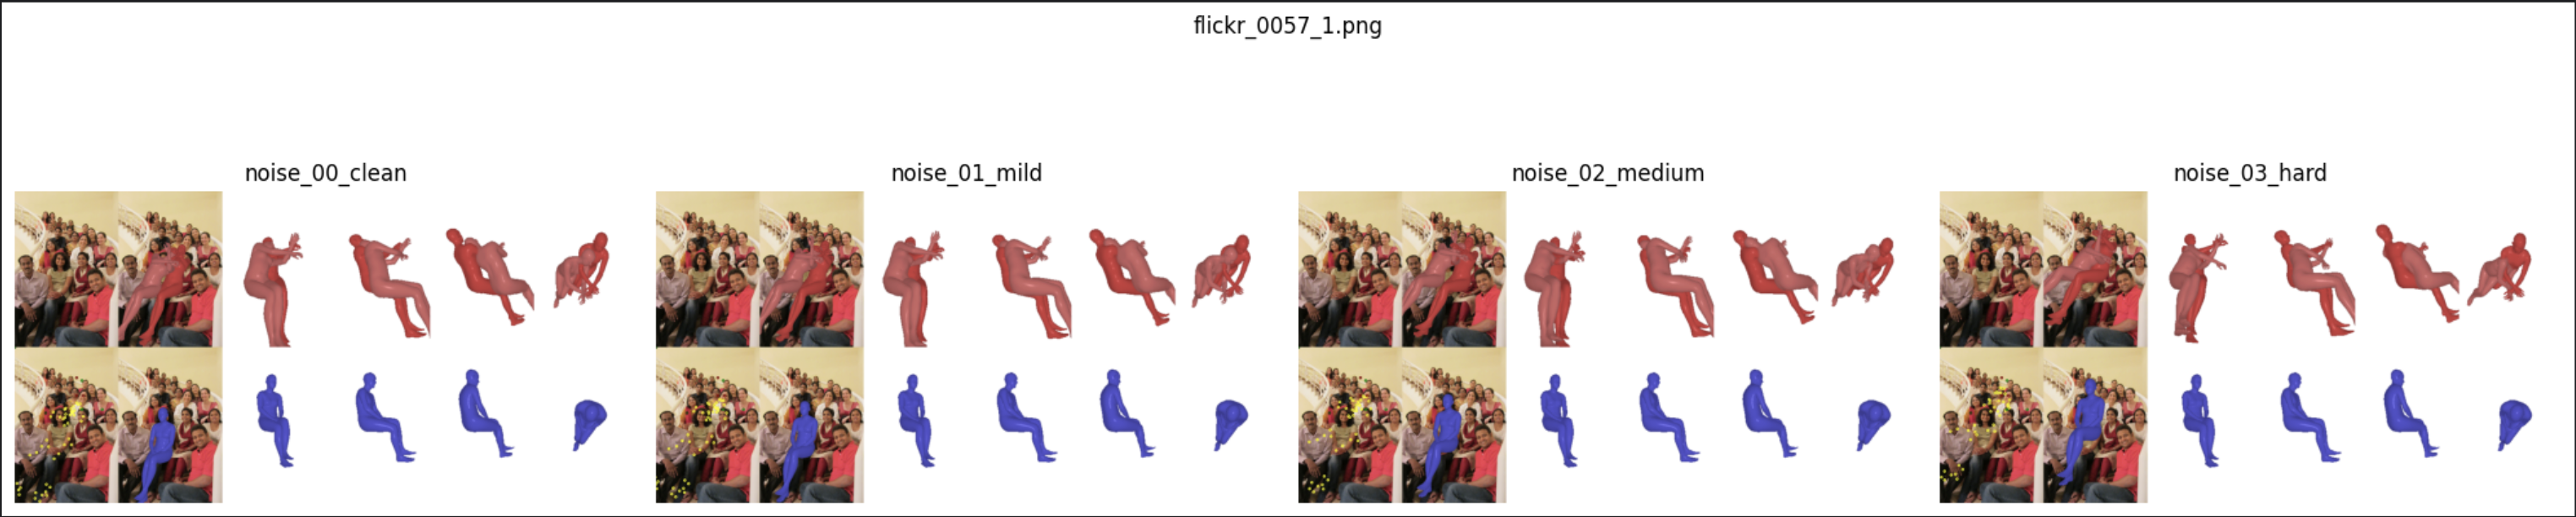
\includegraphics[width=\linewidth]{task3_noise_comparison.png}
    \caption{Qualitative comparison across clean, mild, medium, and hard-noise BEV initializations. This figure should show the same example reconstructed under different initialization noise levels.}
    \label{fig:task3_noise_comparison}
\end{figure}



\section{Discussion}

The Task 3 experiment suggests that BUDDI optimization can still complete when the BEV initialization is degraded. This is consistent with the idea that BUDDI is not merely copying the BEV output, but performs an optimization process using image evidence and a learned prior over two-person interactions.

At the same time, the results must be interpreted carefully. Since the processed FlickrCI3D pseudo-ground-truth files were not accessible, we could not compute official numerical metrics. Therefore, our Task 3 does not prove quantitatively that BUDDI improves noisy BEV reconstructions. It should instead be understood as a qualitative robustness check.

\subsection{What was easy}

Once the environment was working, the high-level structure of the BUDDI pipeline was clear. The demo made it possible to understand the flow from images to ViTPose detections, BEV initialization, and BUDDI optimization. The saved BEV outputs were also readable enough to identify the main fields needed for the noise experiment.

\subsection{What was difficult}

The most difficult part was environment reproduction. The original codebase depends on several packages that are sensitive to Python and PyTorch versions. Running the code on Kaggle required multiple fixes for package compatibility. Another major difficulty was data access: the original FlickrCI3D images were available, but the processed auxiliary files needed for official quantitative evaluation were not accessible.

\subsection{Communication with original authors}

We did not obtain access to the authors' processed FlickrCI3D auxiliary files during the experiment. Because of this, we adapted Task 3 to use the original FlickrCI3D test images and the BEV/ViTPose outputs generated by the demo pipeline.

\section{Conclusion}

We partially reproduced the BUDDI pipeline by successfully running ViTPose, BEV, and BUDDI optimization on FlickrCI3D test images. For Task 3, we implemented a modified robustness experiment by injecting controlled noise into the BEV initialization and rerunning BUDDI optimization for four noise levels.

The experiment produced valid PKL files, OBJ meshes, and visualization images for all noise settings. However, due to the lack of processed pseudo-ground-truth files, the evaluation remains qualitative. A full quantitative reproduction of the robustness study would require access to the authors' processed FlickrCI3D files and official evaluation protocol.

\section*{Member contributions}

\begin{itemize}
    \item \textbf{Teammate 1 Name:} Task 1 -- generator training and unconditional generation evaluation. \textcolor{blue}{Add details.}
    \item \textbf{Teammate 2 Name:} Task 2 -- optimization-based reconstruction and reproduction of main reconstruction results. \textcolor{blue}{Add details.}
    \item \textbf{Nawfal Abdul Malick:} Task 3 -- Kaggle setup, dependency fixes, FlickrCI3D demo execution, BEV output inspection, BEV noise generation, BUDDI reruns under degraded initialization, and qualitative robustness analysis.
\end{itemize}

\bibliography{main}
\bibliographystyle{tmlr}

% Uncomment only if you use appendix.tex
% \include{appendix}

\end{document}